% Tutorial 05

\subsection{Tutorial 5: Accelerated Enveloping Distribution Sampling (AEDS)}

Alchemical free-energy methods have been established as an irreplaceable tool in computational drug design. A vast variety of methods to perform alchemical transformations exists. One family of free-energy methods is the free-energy perturbation (FEP) based on Zwanzig´s equation (eq. \ref{eq:Zwanzig1}) \cite{Zwanzig1954}. Defining the free energy difference $\Delta G_{i,j}$ between two states $i$ and $j$, represented by Hamiltonian's $H_i$ and $H_j$ over the positions $r$ as an ensemble average over state $i$. 

\begin{equation}
\begin{aligned}
\Delta G_{i,j} & = G_j - G_i \\ & = -k_BT \ln  \Biggl \langle e^{ -(H_j(\vec{r}) - H_i(\vec{r}))/k_BT} \biggr \rangle_i 
\end{aligned}
\label{eq:Zwanzig1}
\end{equation}

As mentioned in placeholder sampling relevant phase-space is of utmost importance to converge to plausible results. While methods like TI\cite{kirkwood_TI} or BAR\cite{bar} aim to connect physical states through non-physical states, one-step perturbation methods take a different approach. Here, a reference Hamiltonian, constructed from the end-states, is sampled. This avoids spending simulation time on non-relevant states. This method fits perfectly to investigate closely related systems like derivates. In this tutorial, we will take a look at accelerated enveloping distribution sampling (AEDS) \cite{JP2018,JP2020}. In enveloping distribution sampling a reference Hamiltonian $H_R(\vec{r})$ is constructed by combining several different end-state Hamiltonian's $H_i(\vec{r})$. Since the minimum of each end-state is preserved, $H_i(\vec{r})$ is biased by an offset $\Delta F_{i}^R$. The partition function of $H_R(\vec{r})$ results now as the sum of the biased end-state partition functions (eq. \ref{eq:EDS1}).
%\nameref{equ:ext_ti}
\begin{equation}
\begin{aligned}
H_R(\vec{r}) & = -k_BT \ln  \left( \sum_{i=1}^{N} e^{ -(H_i(\vec{r}) - \Delta F_{i}^R)/k_BT} \right) 
\end{aligned}
\label{eq:EDS1}
\end{equation}

Since this approach can lead to high energy barriers between the minima and thus to sampling problems, the original EDS version introduced a smoothing parameter s (eq. \ref{eq:EDS2}) to smoothen the energy landscape. 

\begin{equation}
\begin{aligned}
H_R(\vec{r}) & = -\frac{k_BT}{s} \ln  \left( \sum_{i=1}^{N} e^{ -(H_i(\vec{r}) - \Delta F_{i}^R)/k_BT} \right) 
\end{aligned}
\label{eq:EDS2}
\end{equation}

This can lead to a deformation of the energy landscape, not preserving the position of the energy minima. Therefore, a refined approach using a boosting potential was proposed \cite{JP2018,JP2020}. Similar to tutorial 4 a harmonic boosting potential is used to accelerate defined regions namely the perturbed atoms and non-bonded interactions. The accelerated reference Hamiltonian $H_R^{\ast}(\vec{r})$ is defined as shown in equation \ref{eq:AEDS}, where the acceleration range is defined by $E_{max}$ and $E_{min}$. 

\begin{equation}
  \begin{aligned}
H_R^{\ast}(\vec{r}) =\begin{cases}
        H_R(\vec{r}) - \frac{E_{max} - E_{min}}{2} &\text{if} \, H_R(\vec{r}) \geq E_{max} \\

        H_R(\vec{r}) - \frac{1}{2(E_{max} - E_{min})}(H_R(\vec{r}) -  E_{min})^2 &\text{if} \,  E_{min} < H_R(\vec{r}) < E_{max} \\

        H_R(\vec{r}) &\text{if} \, H_R(\vec{r}) \leq E_{min} \\
     \end{cases}
  \end{aligned}
  \label{eq:AEDS}
\end{equation}

To obtain parameters for $E_{max}$, $E_{min}$, and the offsets a parameter search simulation is a necessity. In the search simulation, the currently sampled state is defined as the state with the lowest energy for $H_i(\vec{r}) - \Delta F_{i}^R$. $E_{max}$ is defined as the maximum observed transition energy after a full state round trip, meaning that each state was sampled at least once. $E_{min}$ is based on the fluctuations of $H_i(\vec{r})$ of the state with the lowest energy. The offsets have different definitions depending on the search algorithm in use. Generally, the difference between two offsets $\Delta\Delta F_{ij}$ is the free energy difference between the accelerated end-states $i$ and $j$. In older iterations of the search algorithm, the offsets were estimated as the free energy difference between an accelerated end-state and the accelerated reference state and afterward anchored to one of the end-states. The search algorithm used in this tutorial uses an approach similar to local elevation by continuously adding to the offsets based on the contribution to the free energy. In this approach, all offsets are averaged around zero. This has proven to be a more robust search algorithm and removed the dependency on the anchor state. The parameters obtained from the search simulation are then used in a production run.

\subsubsection{Preparations}
In this tutorial, we will use two SPC water molecules as a test system. We will use AEDS to calculate free energy differences and as a tool for water probing in a protein-ligand system \cite{gracia1}.   
 
The preparation of the topology, coordinates, energy minimization, and equilibration of the system follows the same procedure as described in tutorial 1.
The final equilibrated structures can be found in the directory \texttt{eq}. The perturbation topologies can be created as shown in tutorial 2 and are provided in the directory \texttt{topo}.

\subsubsection{Acceleration parameter search}
To get the acceleration parameters ($E_{max}$, $E_{min}$, offsets) a search simulation needs to be performed. The search run starts from an equilibrated structure. If no initial parameters are given the search starts as a conventional MD simulation. After each simulation step $E_{max}$, $E_{min}$, and the offsets are updated. After approximately 5-25 ns the parameter search simulation converges. The needed simulation time depends mostly on the complexity of the system and the perturbation since we are dependent on visiting all end-states to adjust the acceleration parameters. In this tutorial, we will run a very short search simulation of 0.5 ns and use parameters from a longer simulation for the production run.  

Go to the directory \texttt{search}. In this folder, you will find three files namely \texttt{aeds.arg}, \texttt{aeds.job}, and \texttt{aeds.imd}. Let's start with the \texttt{aeds.imd} file. This file is a simulation input file we already know from previous tutorials. At the bottom of the file, we have an additional AEDS block.
\begin{lstlisting}
AEDS
# AEDS
     1
# FORM  NUMSTATES
     5          4
# EMAX  EMIN
     0     0
# EIR [1..NUMSTATES]
    0   0   0   0 
# NTIAEDSS  RESTREMIN   BMAXTYPE    BMAX 
         1          1         2        2    
# ASTEPS    BSTEPS
    1000     10000 
END
\end{lstlisting}
In the second line, we set $FORM$ to 5 specifying an all-parameter search using the adaptive search.
Later we will change this into $FORM$ 1 to run a production run. Other options are described in the  \texttt{gromos} handbook. $NUMSTATES$ specifies the number of end-states in this simulation. Since we perturb two SPC water molecules A and B we get four possible end-states as all combinations of A and B being present or dummies as shown in table \ref{tab:states}.

\begin{table}[h!]
    \begin{center}
     \begin{tabular}{*{3}{m{0.1\textwidth}}}
      & \hfil A & \hfil B \\
       \toprule
        end-state 1
      & 
        \begin{center}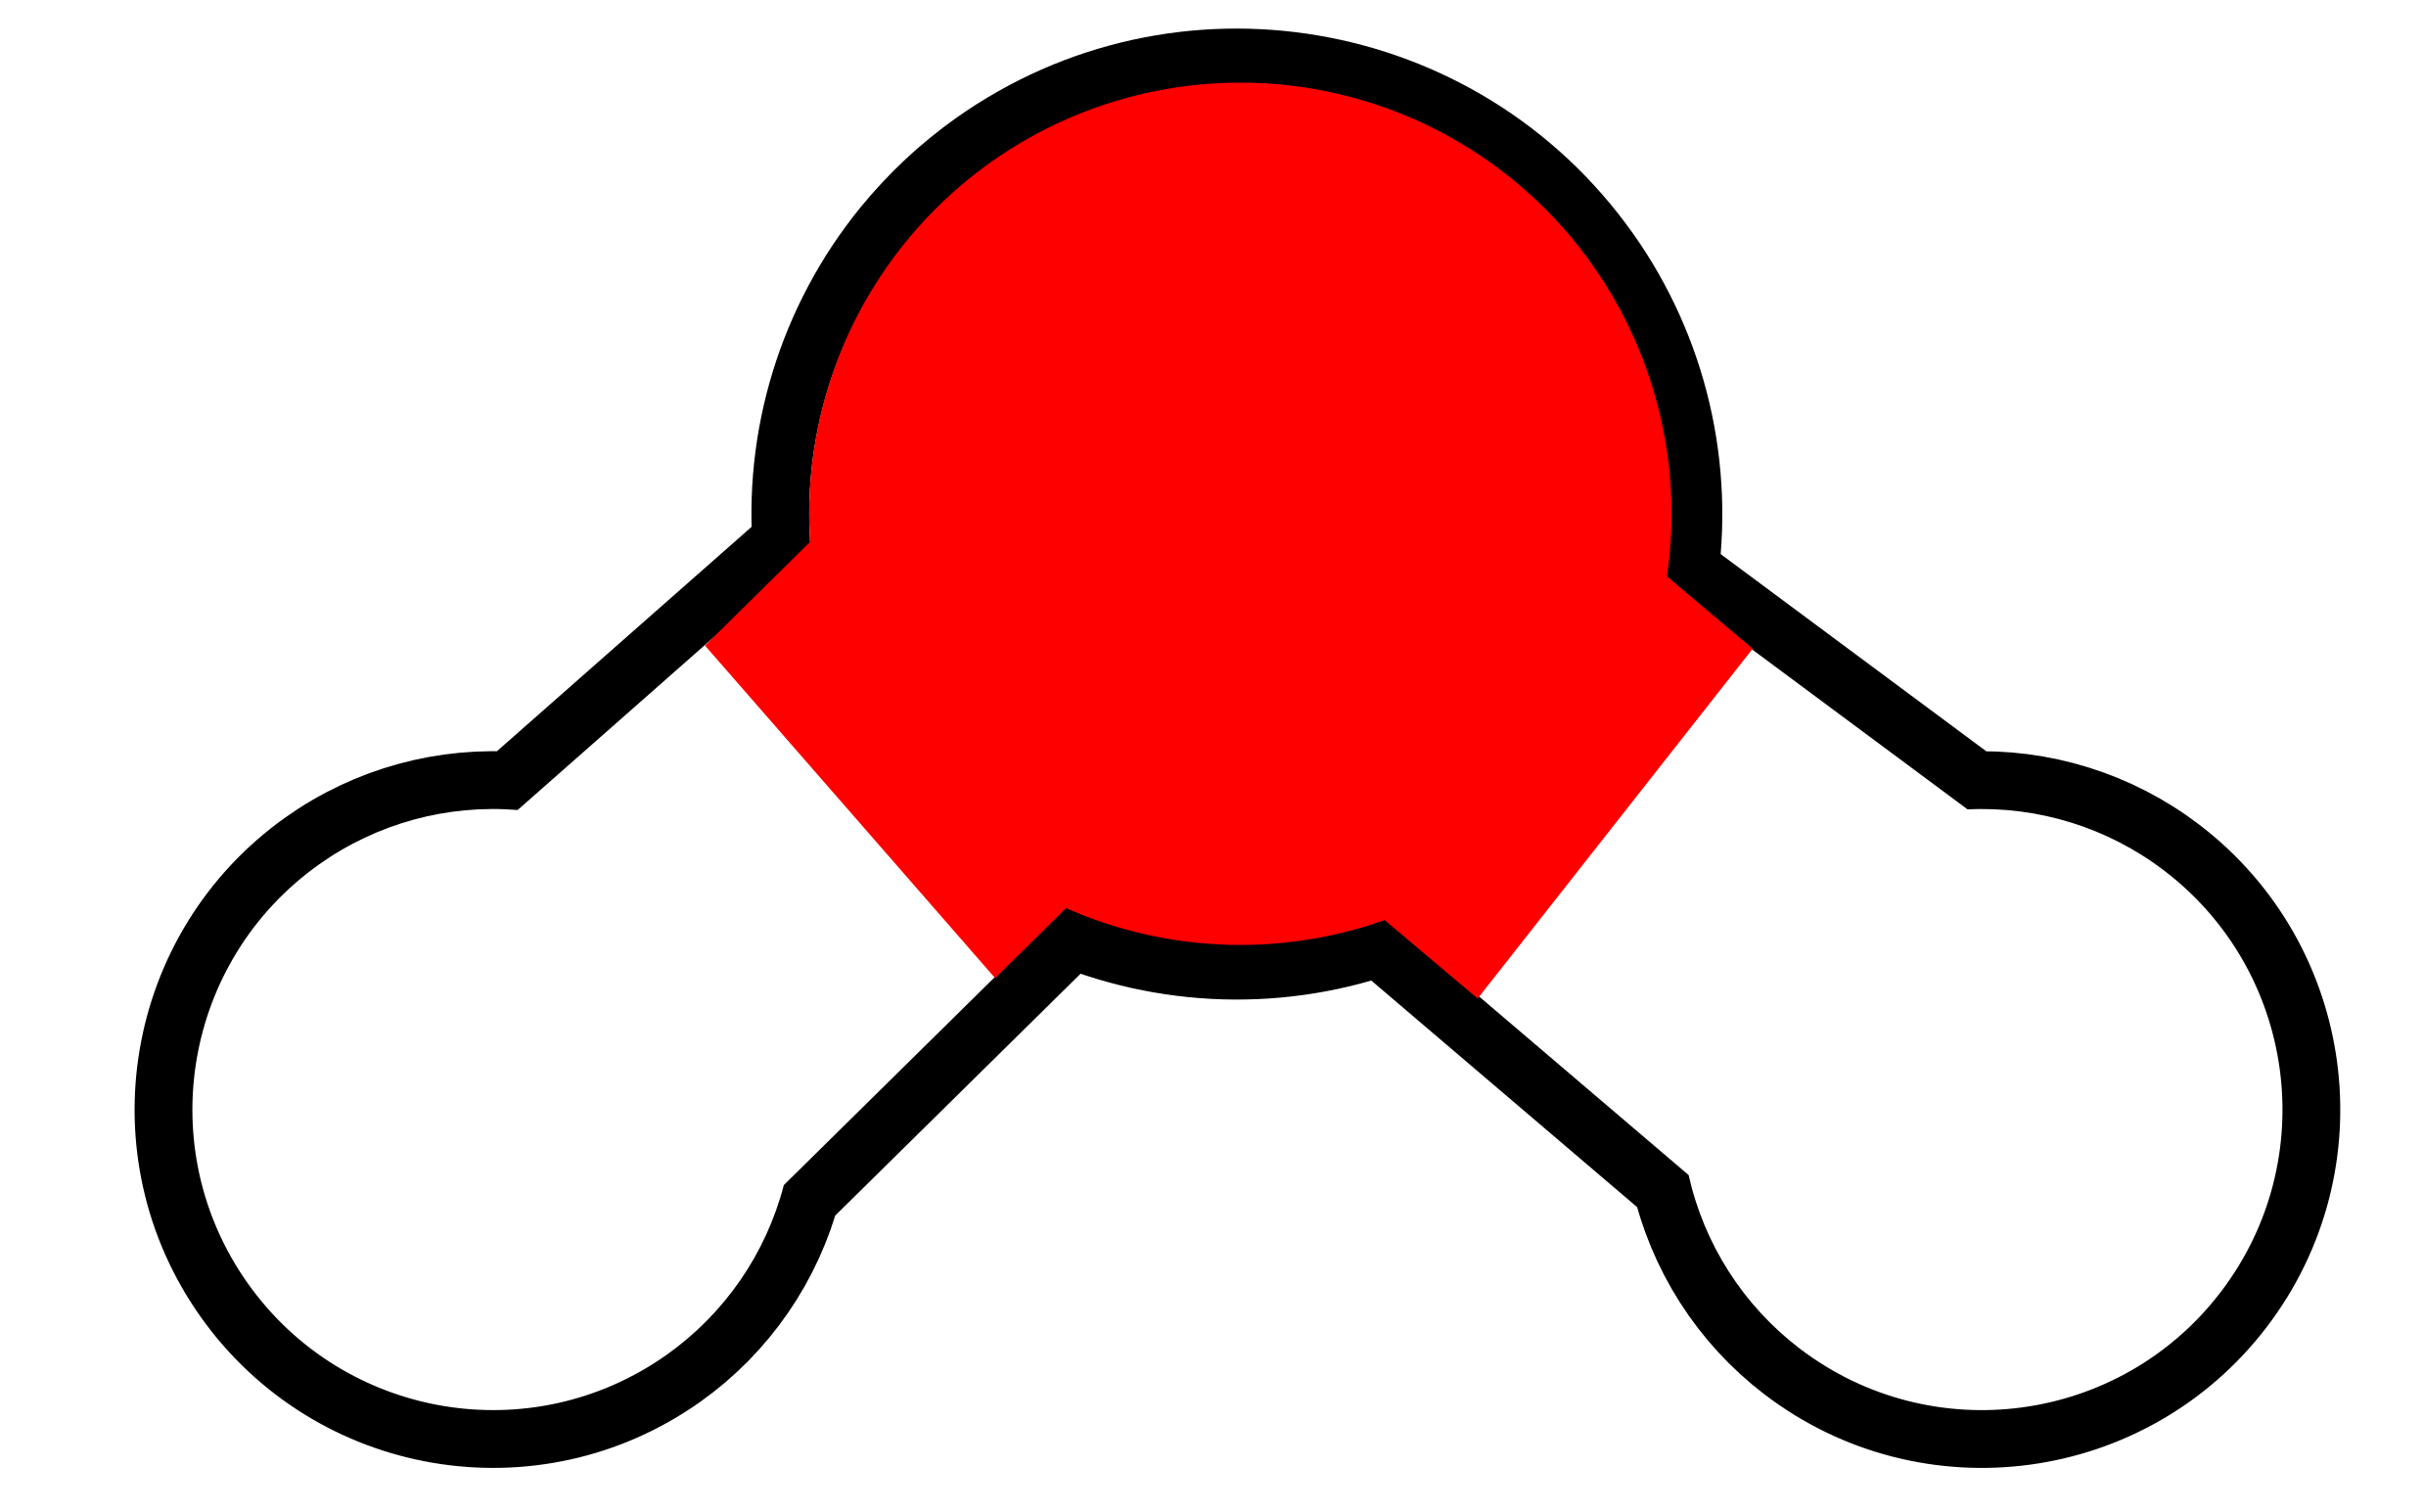
\includegraphics[width=0.08\textwidth]{../08_tutorial_05/figures/water.png}\end{center}
      & 
        \begin{center}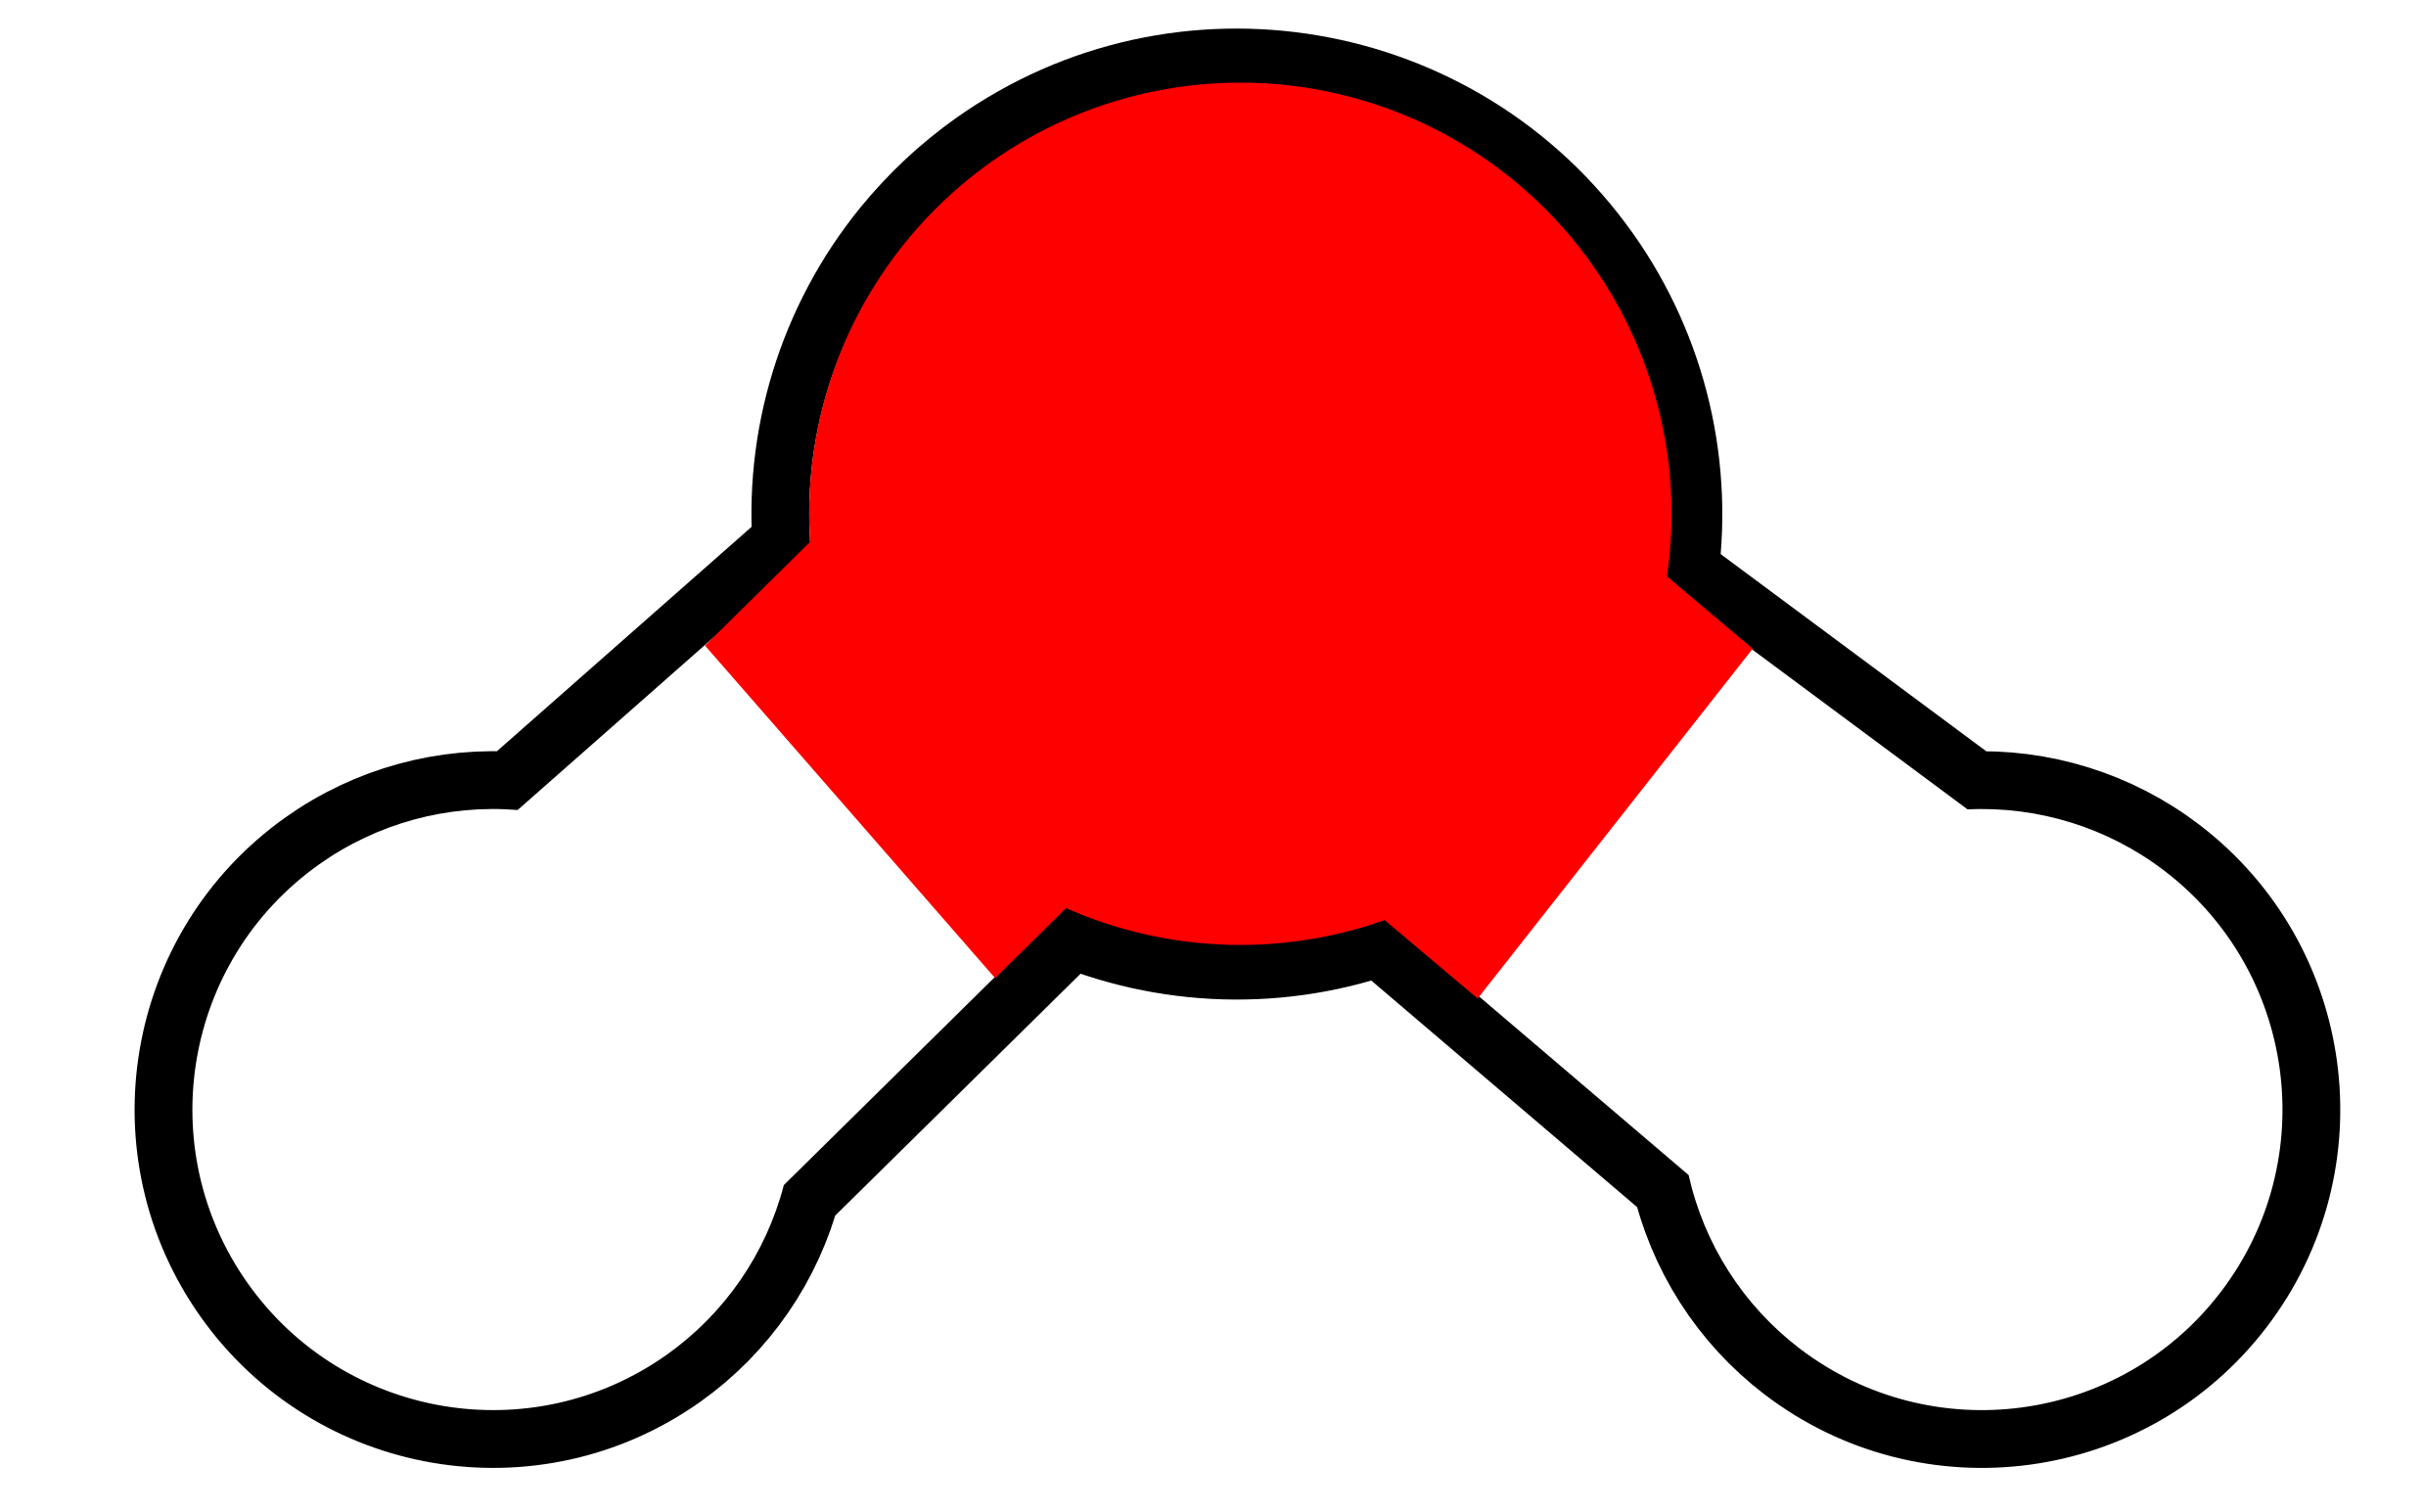
\includegraphics[width=0.08\textwidth]{../08_tutorial_05/figures/water.png}\end{center} \\
        end-state 2
      & 
        \begin{center}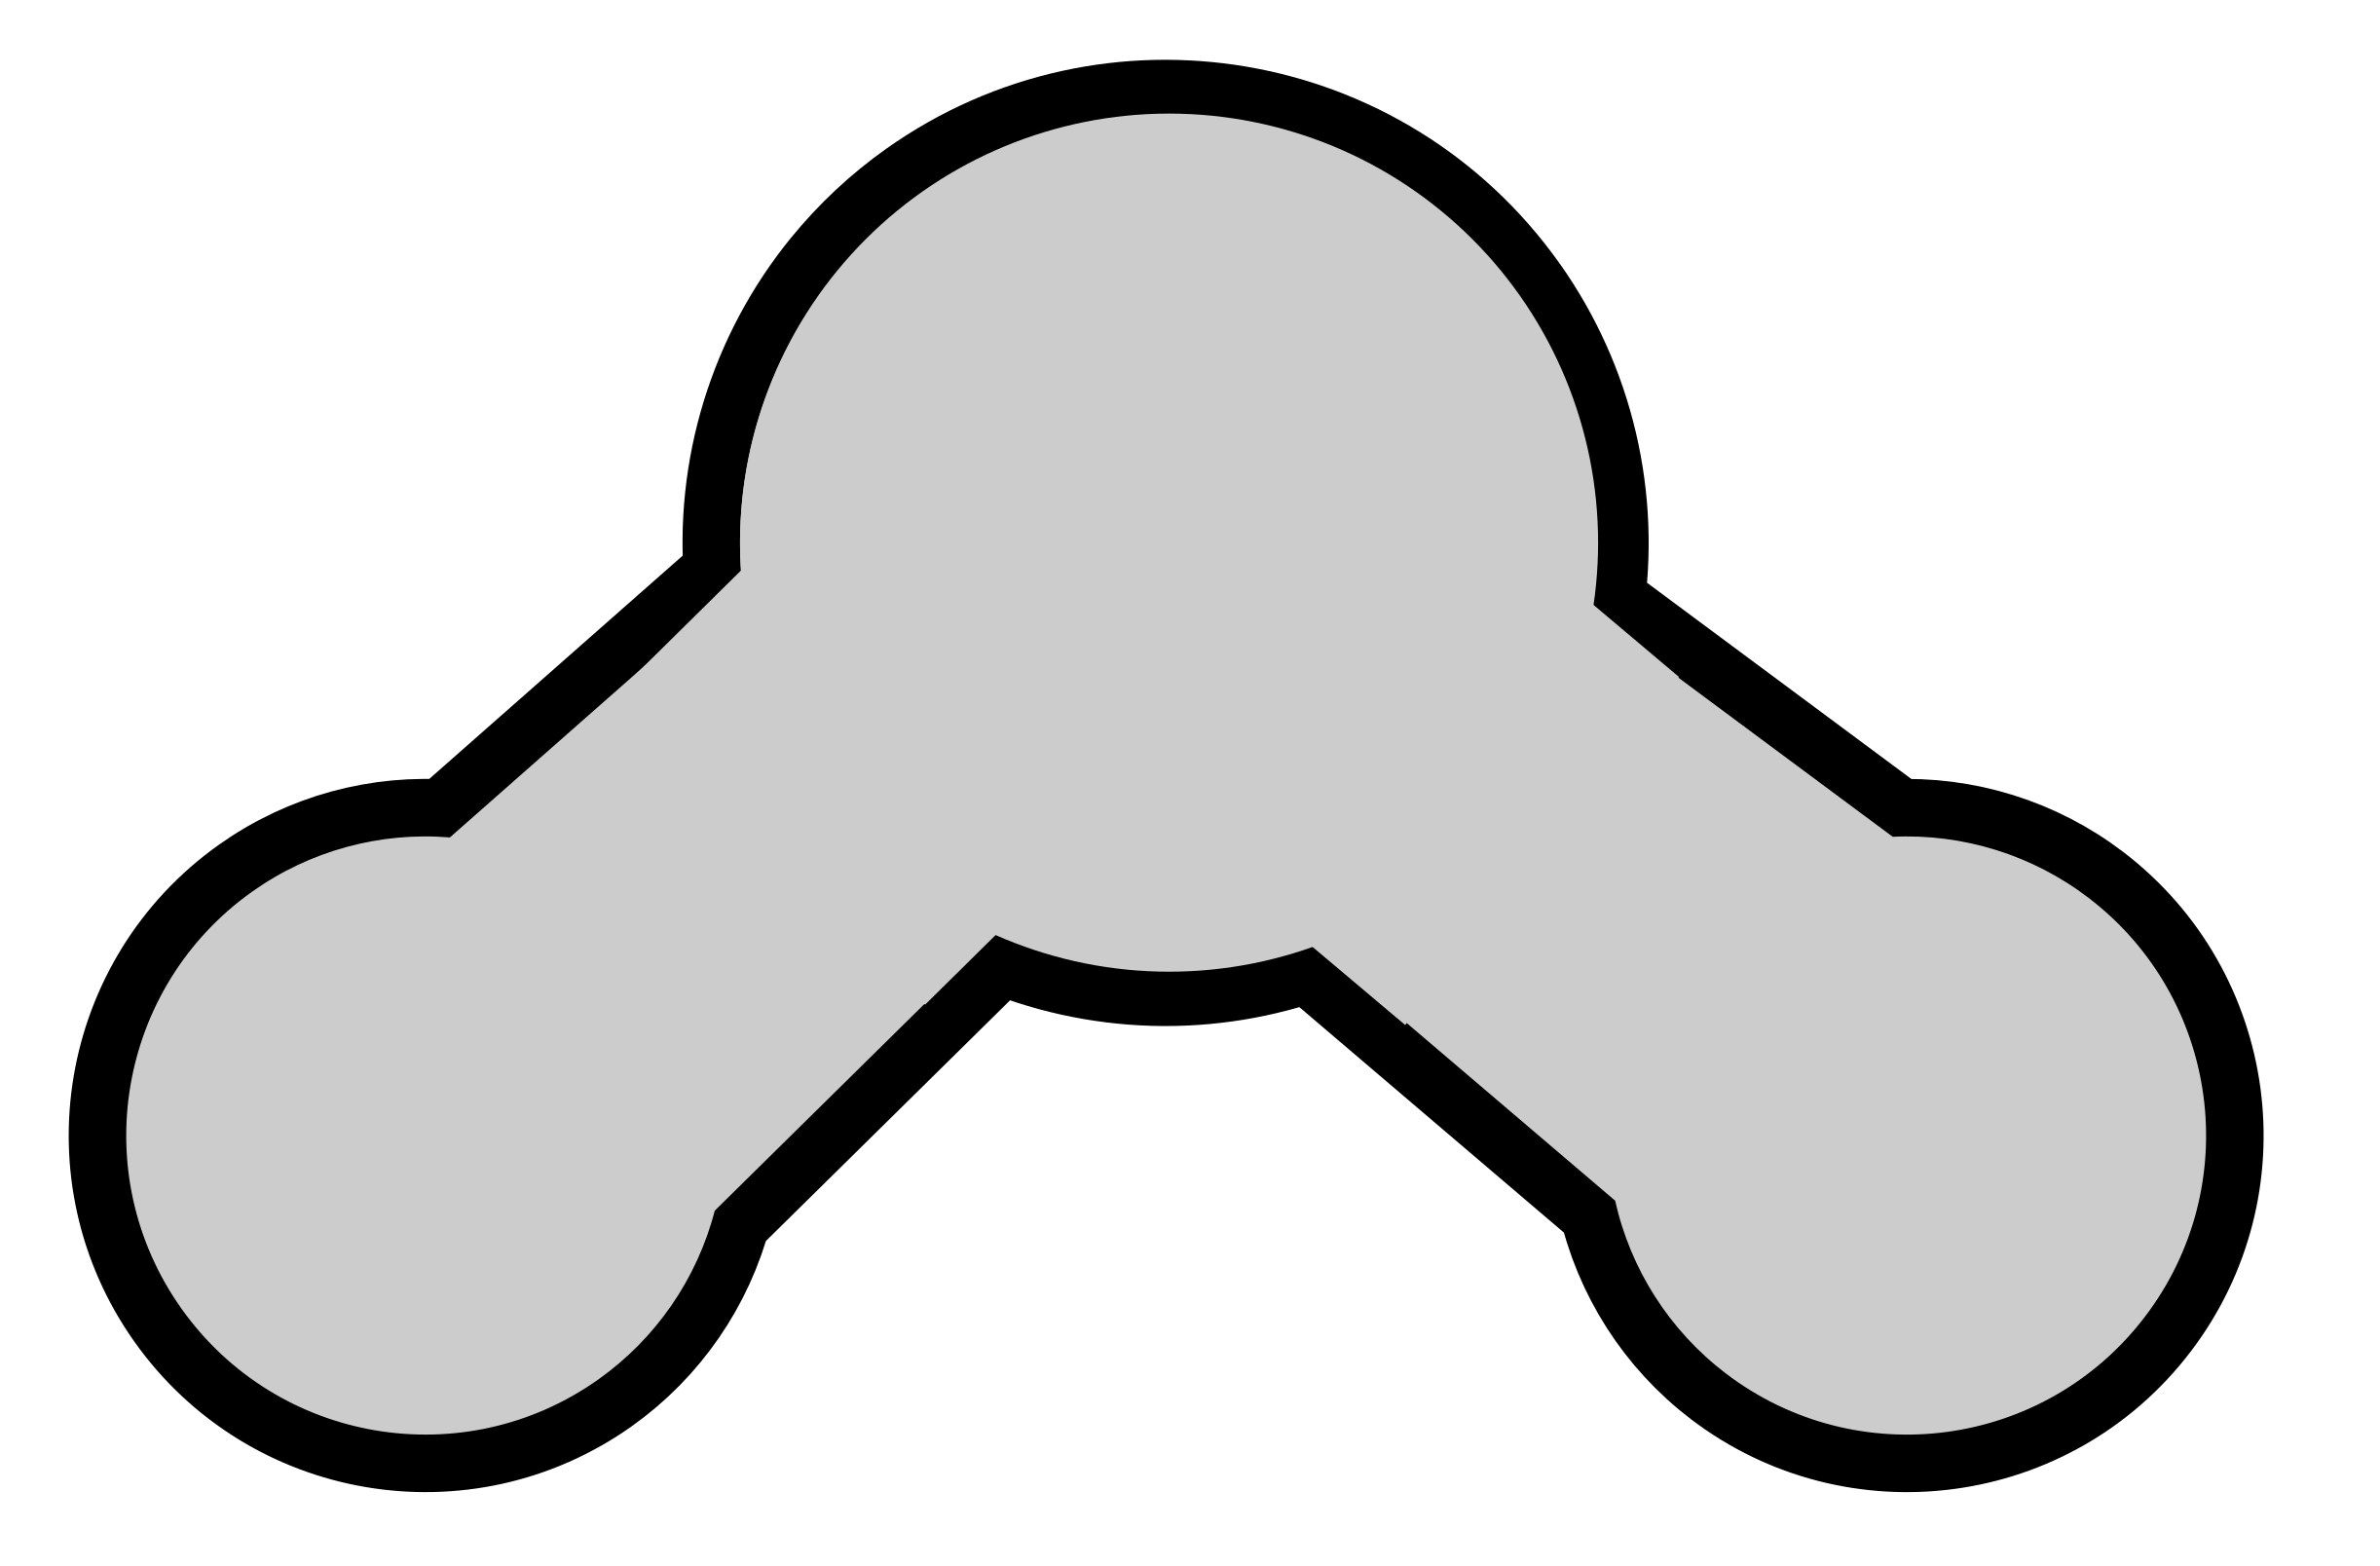
\includegraphics[width=0.08\textwidth]{../08_tutorial_05/figures/dummy.png}\end{center}
      & 
        \begin{center}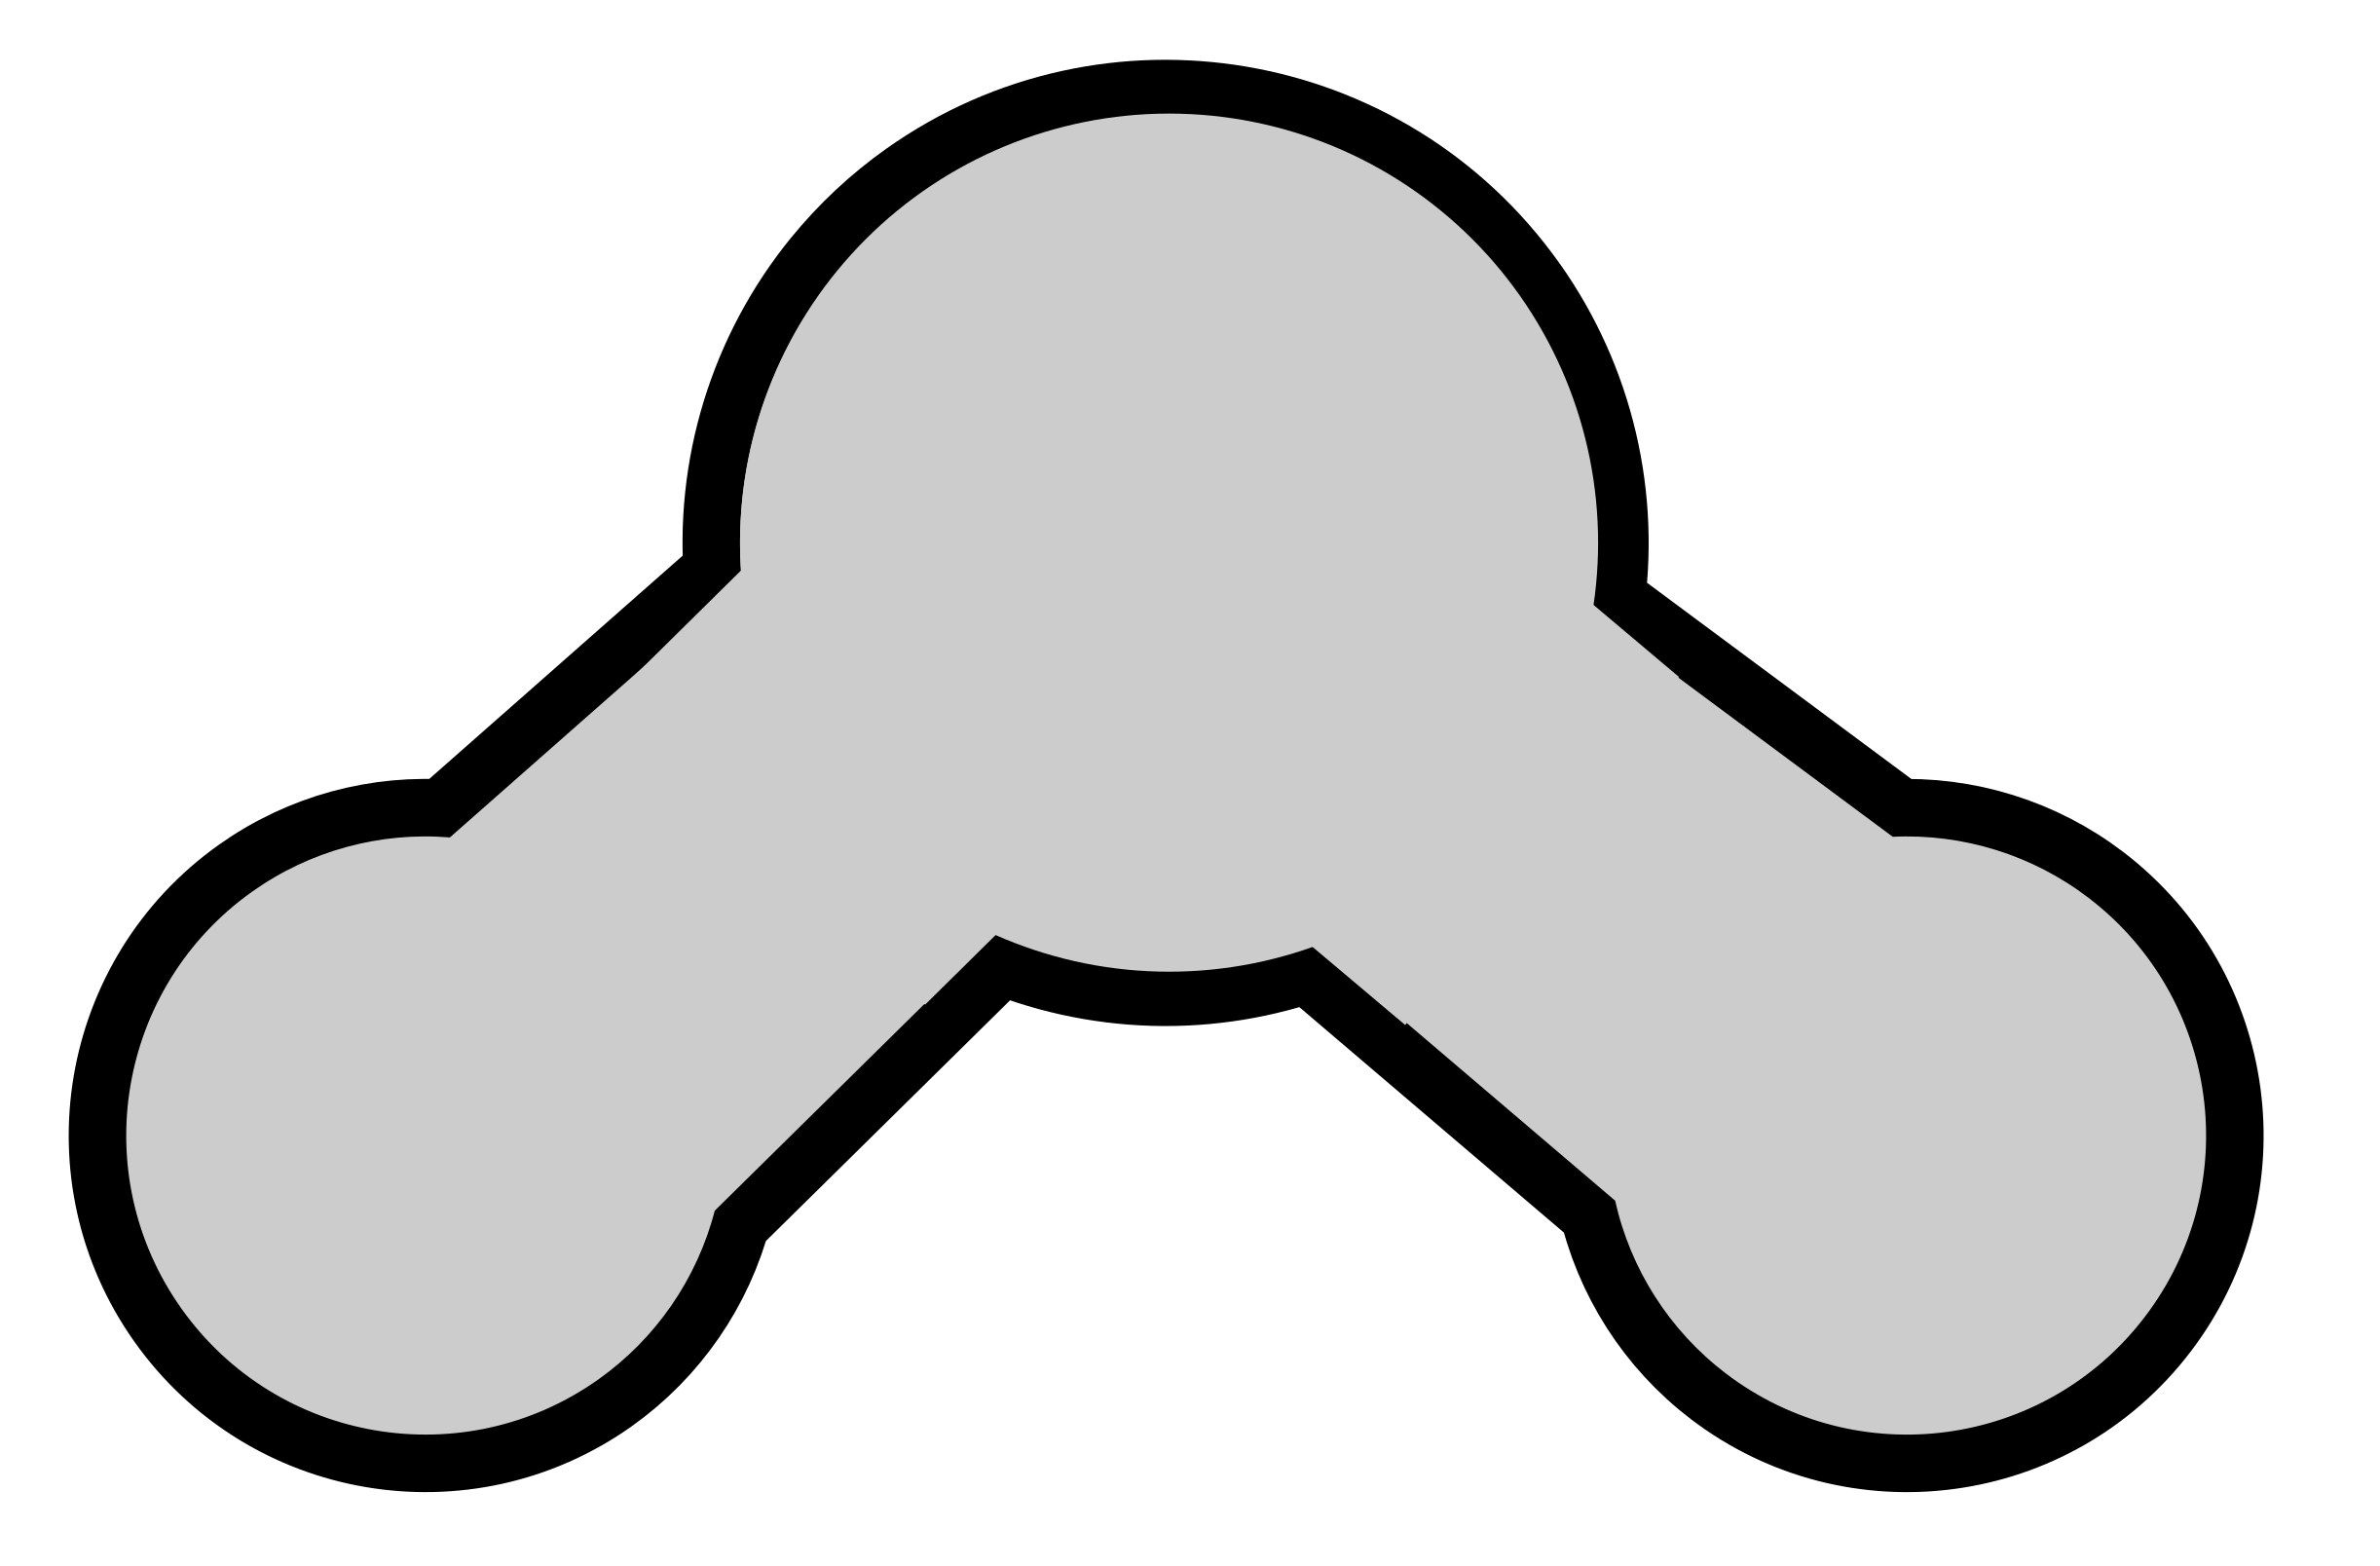
\includegraphics[width=0.08\textwidth]{../08_tutorial_05/figures/dummy.png}\end{center} \\
        end-state 3
      & 
        \begin{center}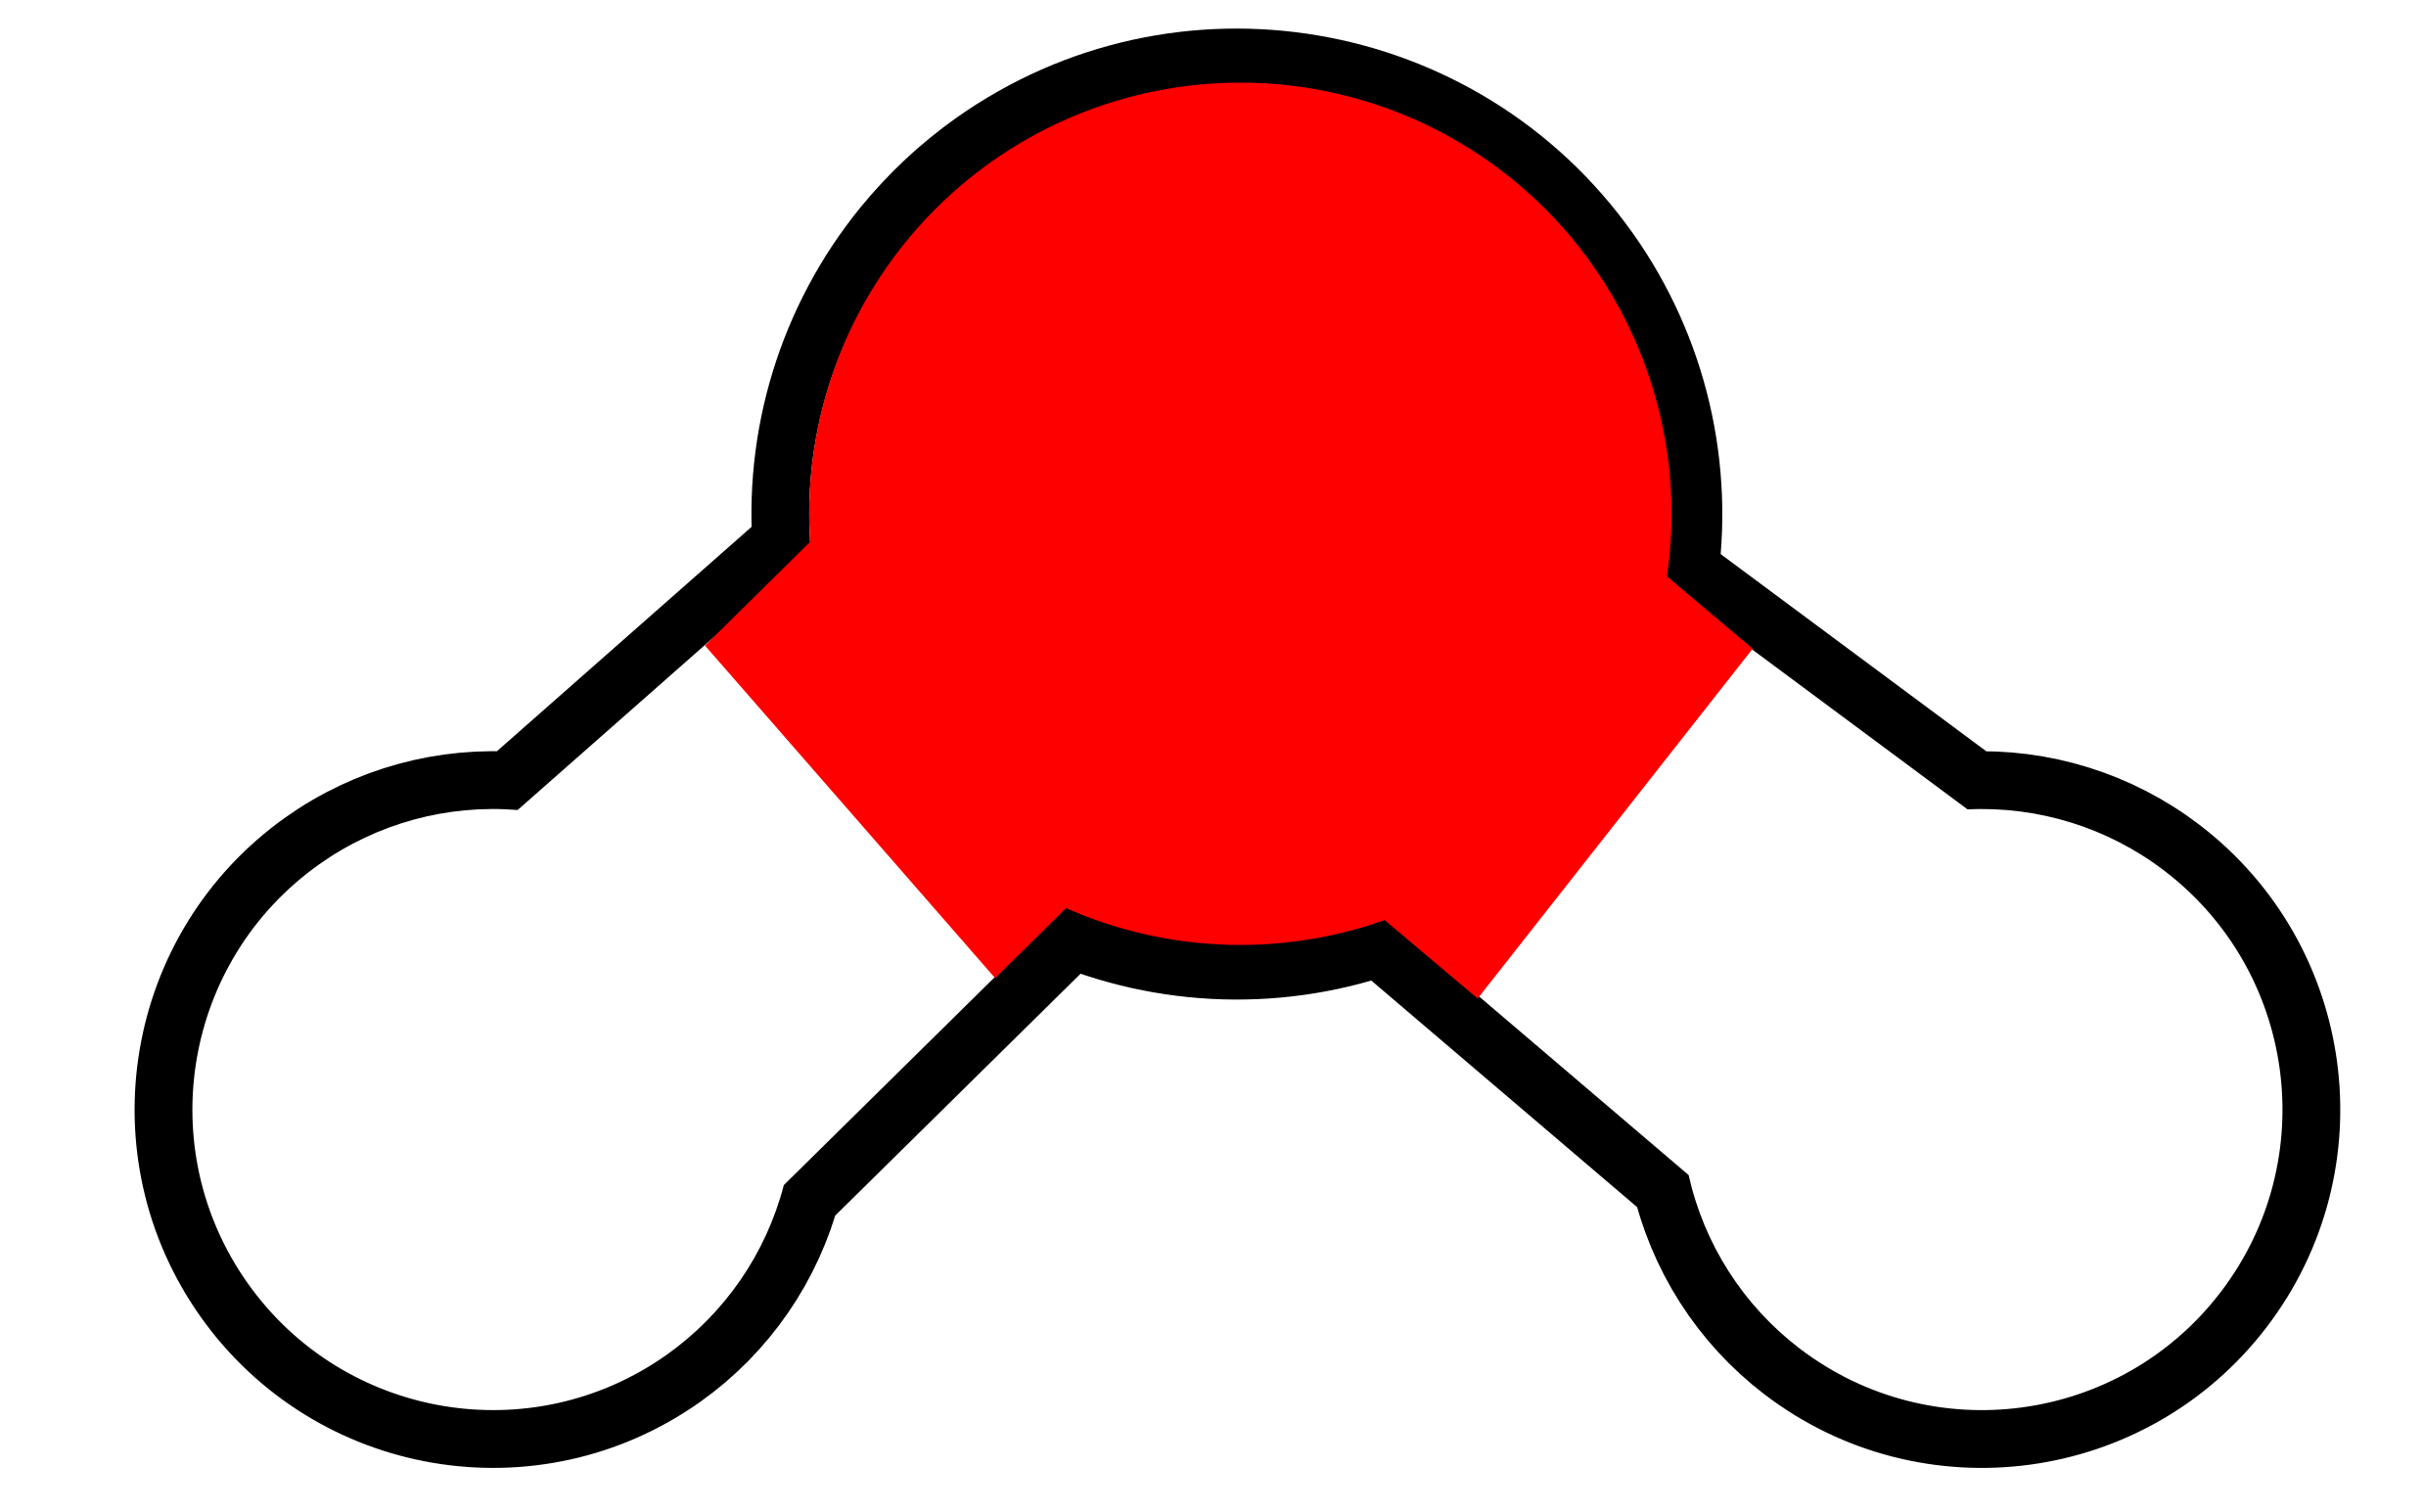
\includegraphics[width=0.08\textwidth]{../08_tutorial_05/figures/water.png}\end{center}
      & 
        \begin{center}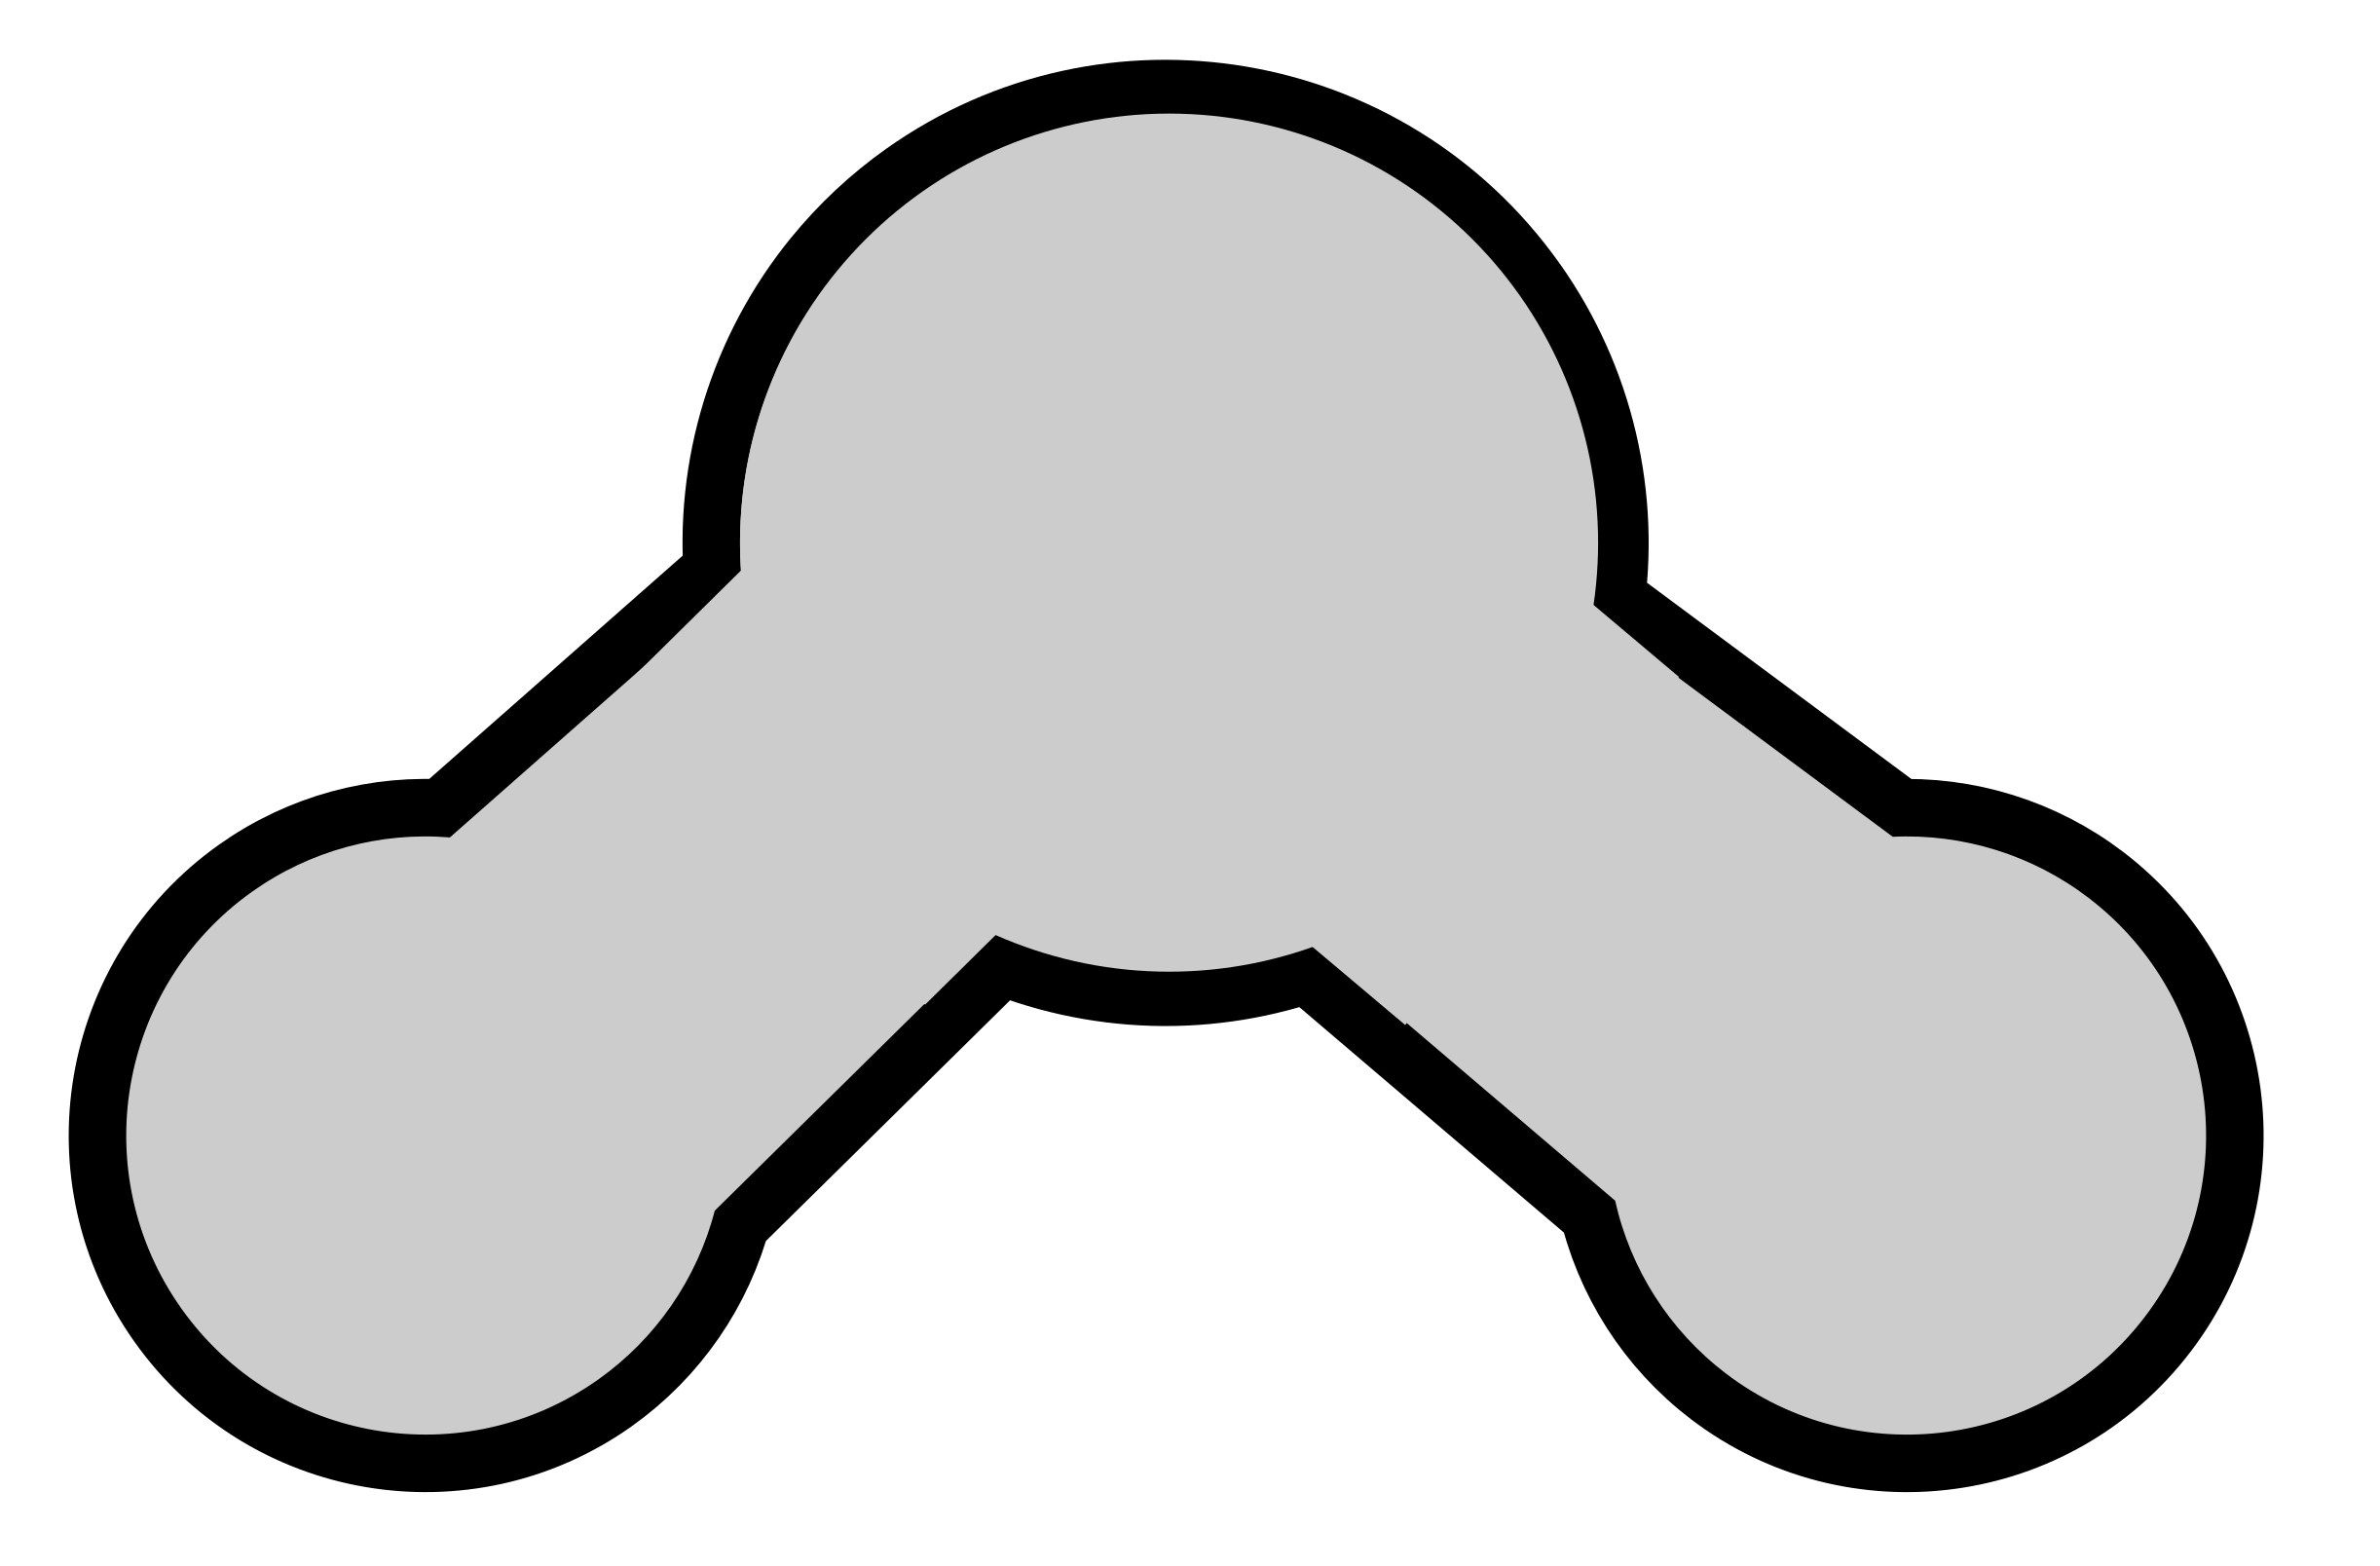
\includegraphics[width=0.08\textwidth]{../08_tutorial_05/figures/dummy.png}\end{center} \\
        end-state 4
      & 
        \begin{center}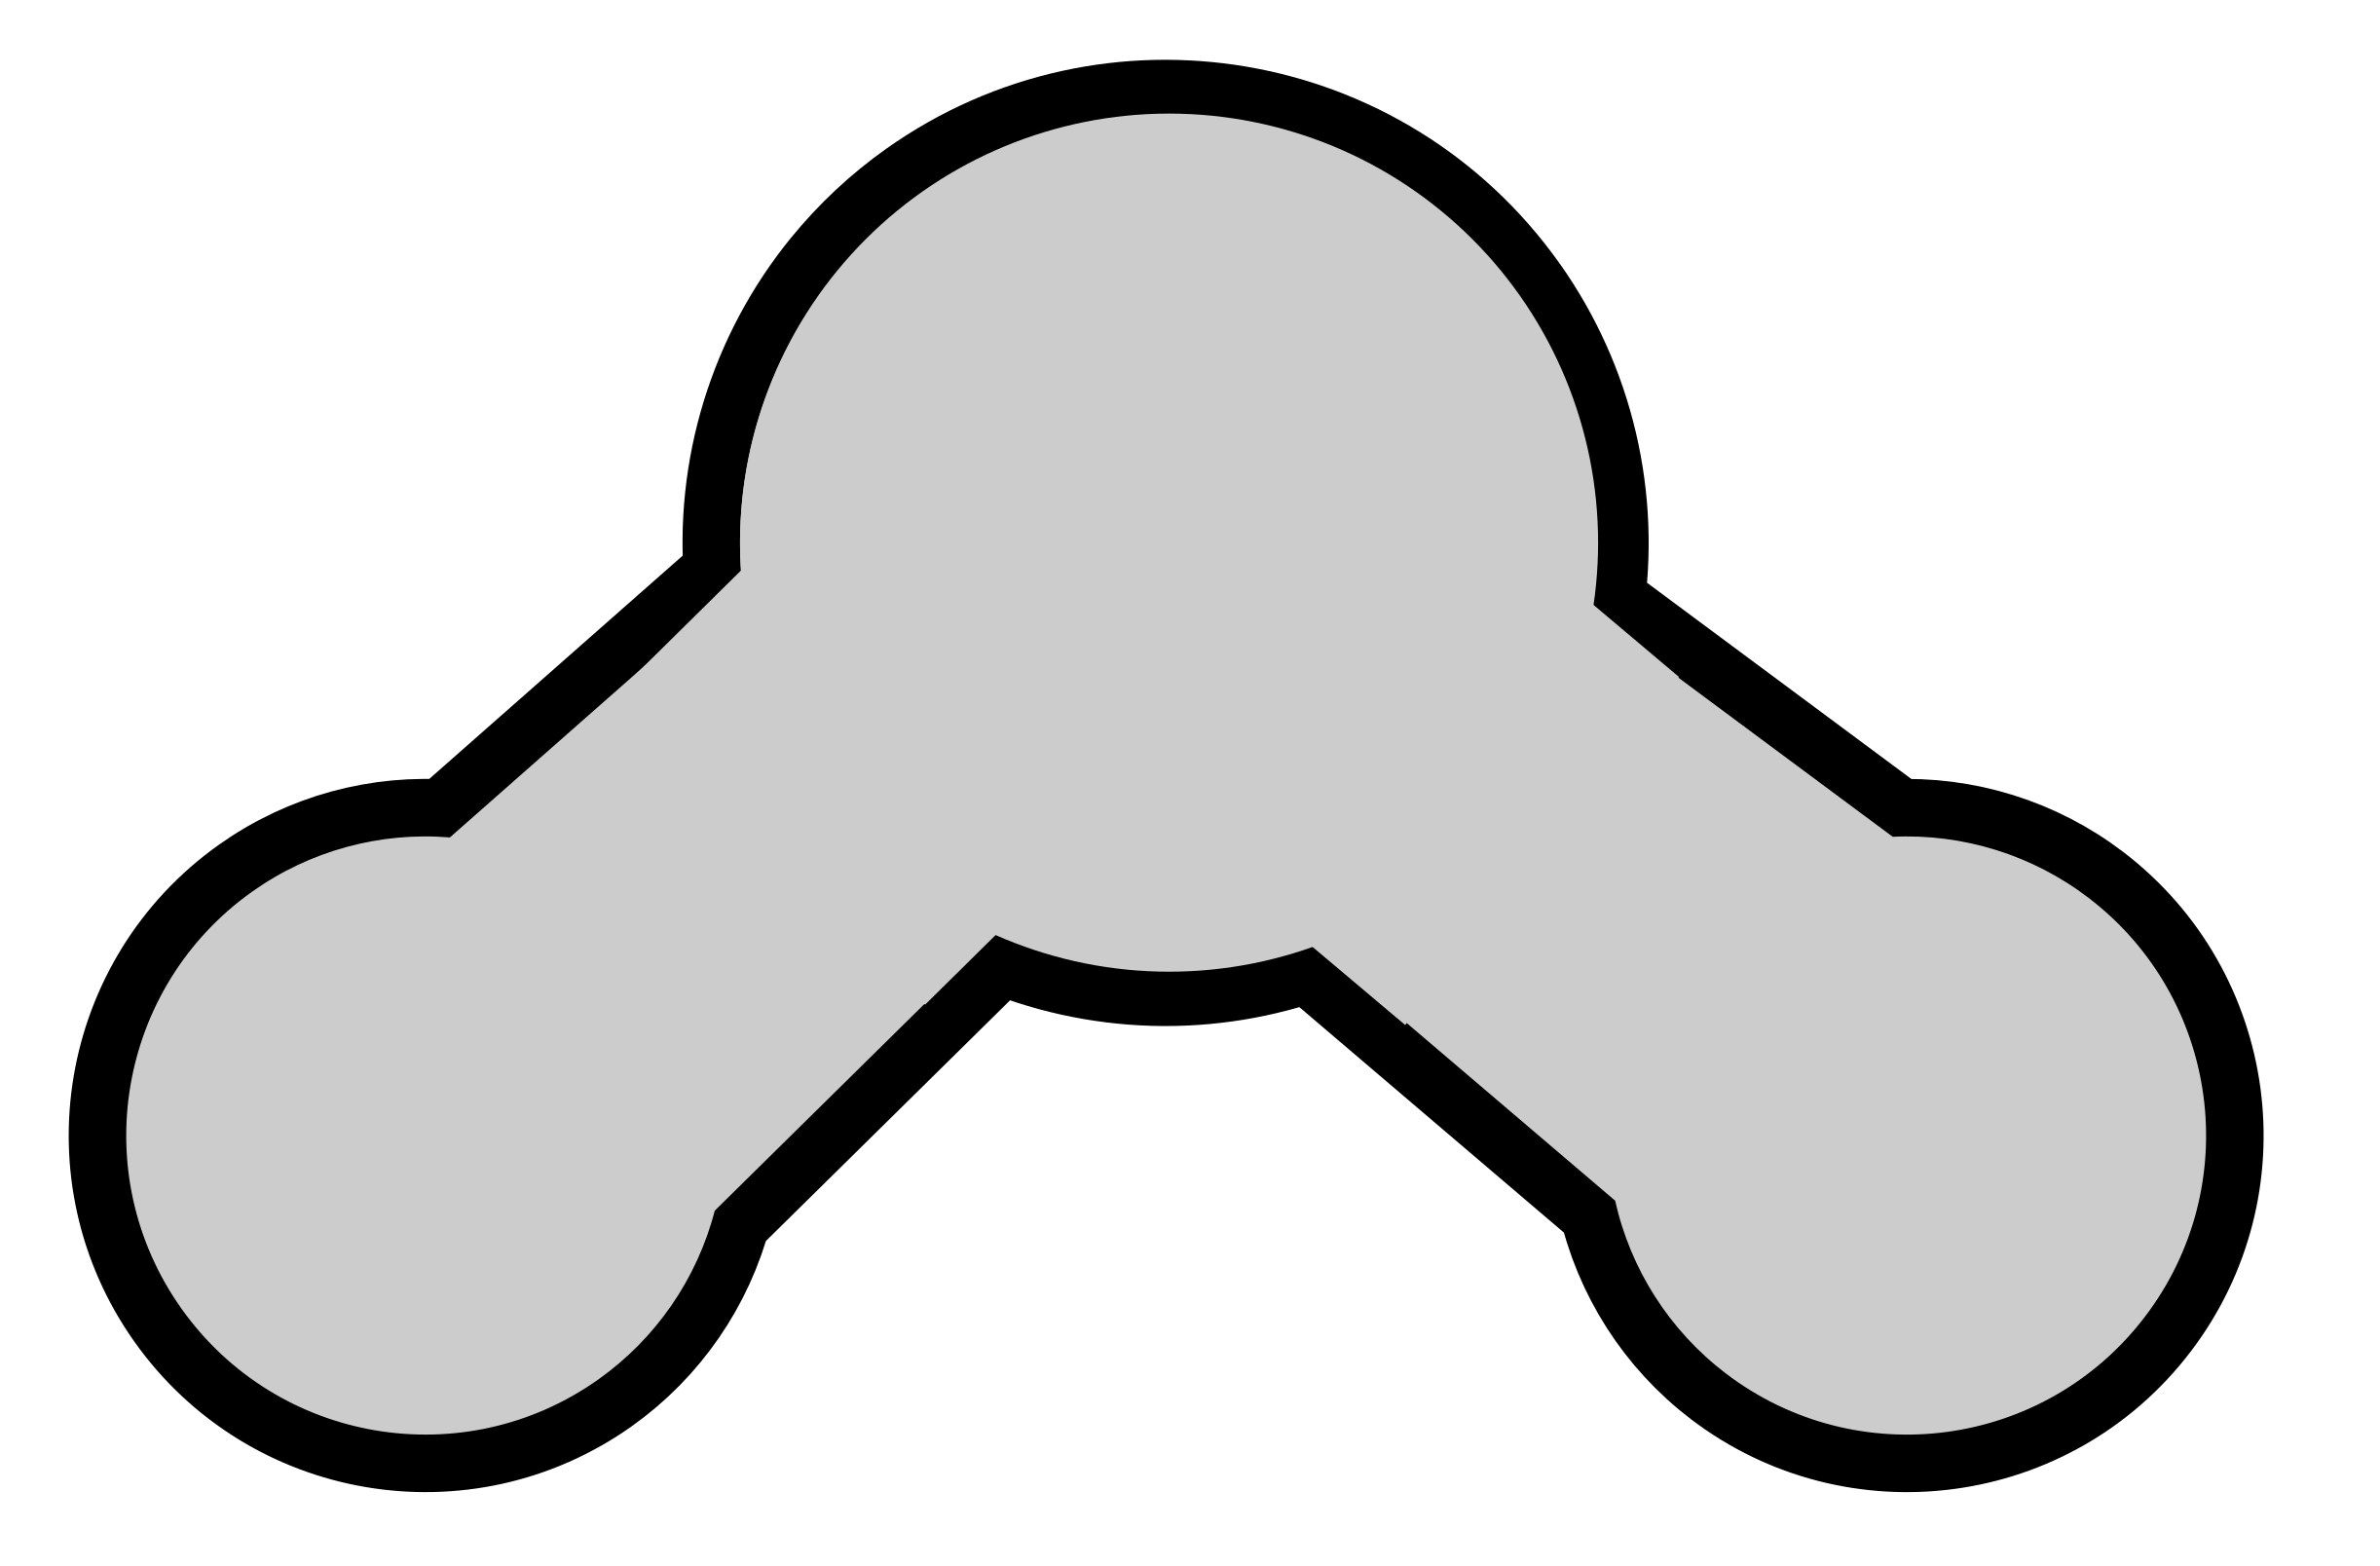
\includegraphics[width=0.08\textwidth]{../08_tutorial_05/figures/dummy.png}\end{center}
      & 
        \begin{center}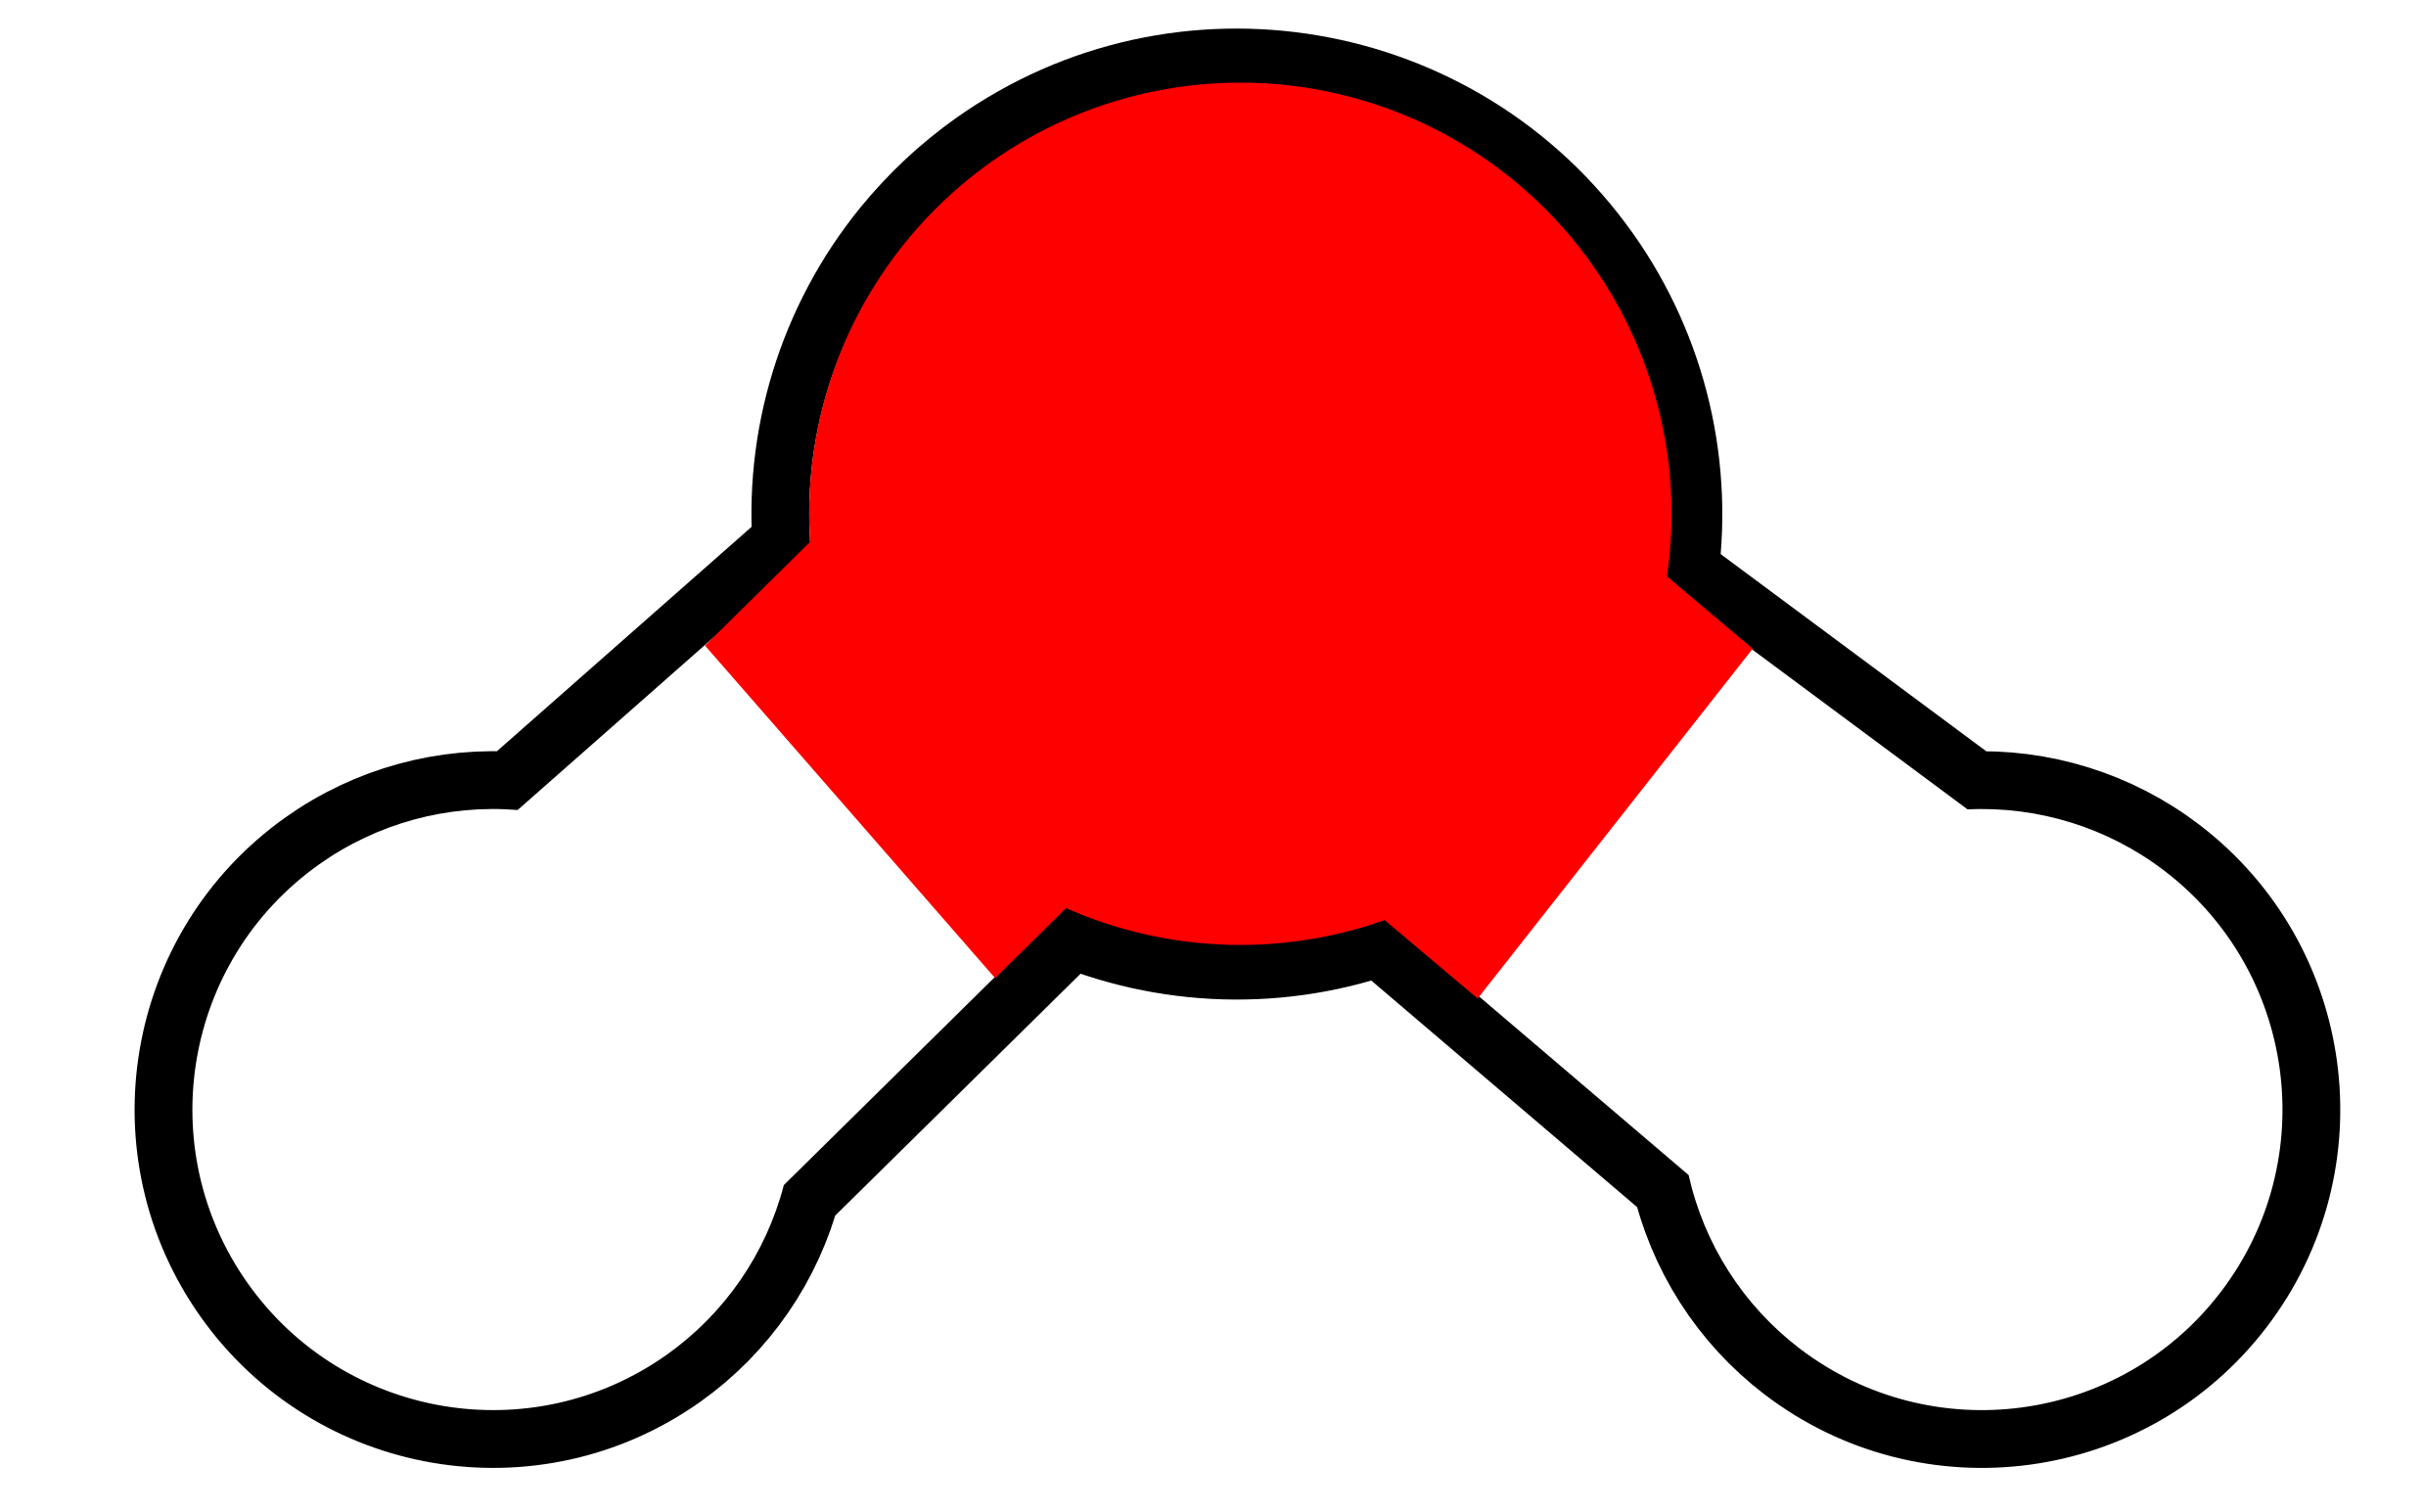
\includegraphics[width=0.08\textwidth]{../08_tutorial_05/figures/water.png}\end{center} \\
      \bottomrule
      \end{tabular}
      \caption{Showing the resulting end-states 1-4 for the perturbation of two SPC water molecules A and B.}
      \label{tab:states}
    \end{center}
\end{table}

In the third line, we set zeros for both $E_{max}$ and $E_{min}$ as well as for the offsets in the line underneath. If we had prior information about these values we could give them as a starting point for the search instead of starting from scratch. Line five is specific for search runs. With $NTIAEDSS$ 1 we initialise the search run. You will see that we turn it off in the jobscript after the first initialization. $RESTREMIN$ restricts $E_{min}$ to the minimum average end-state energy before all states have been visited at least once. $BMAXTYPE$ and $BMAX$ are used to control the estimated maximum barrier height. By default, we set both of them to 2. $ASTEPS$ is used to control the change rate in offsets. A higher number means a faster change in offsets. $BSTEPS$ is used for initial free-energy guesses in other search algorithms. In the argument file, we need to specify the folder location and the location of the md binaries as absolute paths. The \texttt{imd} file uses the $INNERLOOP$ block for \texttt{CUDA} support. If the used \texttt{gromos} binary does not support \texttt{CUDA}, comment the line out using a hashtag. The jobfile is used to create ten \texttt{imd} and \texttt{run} files of the same simulation length as specified in \texttt{aeds.imd}. The only changes in the settings are that 
$NTIAEDSS$ is set to zero after the first jobscript.

With all input files prepared, we can now generate the run files using \texttt{mk\_script} from \texttt{gromos++} package with:
\begin{lstlisting}
$ mk_script @f aeds.arg
\end{lstlisting}

For this tutorial, we provide two \texttt{mk\_script} libraries, one to prepare the run files for a cluster using SLURM as a queueing system (\texttt{libs/mk\_script.lib}), and one for running the simulations locally, (\texttt{libs/mk\_script\_local.lib}).

After running the parameter search simulation, we can extract the acceleration parameters by using \texttt{ene\_ana}. The analysis files are provided in the subfolder \texttt{ana} in the search directory. 
We will use this program to read out the energy and offset of each end-state as well as $E_{max}$ and $E_{min}$. 

You can run the program with 
\begin{lstlisting}
$ ene_ana @f ene_ana.arg
\end{lstlisting}

The file \texttt{ene\_ana.arg} contains the information of which parameters to extract from the defined energy trajectories. The definitions of those parameters can be found in the library file \texttt{libs/ene\_ana.md++.lib}. \texttt{ene\_ana} will generate trajectories of the selected parameters. We could plot \texttt{eds\_emin.dat}, \texttt{eds\_emax.dat}, and \texttt{e*r.dat} to check for convergence, where the \* in \texttt{e\*r.dat} is to be replaced by the end-state number. These files contain the offsets for each end-state. Another way is to use \texttt{search.py} in the scripts folder. This script splits the trajectories into ten blocks and gives us the average $E_{min}$ and $E_{max}$ of the last block in the first line. Underneath the offsets with an error estimate for each end-state averaged for each block are shown. It also calculates the theoretical offsets, as the free-energy difference to the accelerated reference state, shown in the third column. In an ideal case, the offset values converge to a single value in the later blocks and have a small error estimate. In addition, they should be similar to the theoretical offset meaning the free energy difference between the accelerated end-state and the accelerated reference state. Keep in mind that the offsets in column one are averaged around zero.
To call \texttt{search.py} in the \texttt{search/ana} folder , do the following:

\begin{lstlisting}
$ python ../../scripts/search.py
\end{lstlisting}

The output from the longer search run can be found in \texttt{search/ana/long}.
We will use $E_{min}$ and $E_{max}$ as well as the offset parameters from the last block of each end-state found in \texttt{search.out}.

\subsubsection{AEDS production run}
With the parameters from the search run, we can now start a production run. From the production run, we can calculate our relative free energies. Go into the directory \texttt{prod}. Here we see two files, \texttt{aeds.arg} and \texttt{aeds.imd}. We do not use the $@joblist$ argument in the argument file, but the $@script$ argument to specify the number of jobs. If we take a short look into \texttt{aeds.imd} we will spot a few differences:

\begin{lstlisting}
AEDS
# AEDS
     1
# FORM  NUMSTATES
     1          4
# EMAX  EMIN
    43.08  -187.95
# EIR [1..NUMSTATES]
 16.32   -43.66   12.99    14.35 
# NTIAEDSS  RESTREMIN   BMAXTYPE    BMAX   
         0          1         2        2      
# ASTEPS    BSTEPS
    1000     10000 
END
\end{lstlisting}

We now use $FORM$ 1 for a production run. We also inserted values for $E_{max}$, $E_{min}$, and the offsets. We also set $NTIAEDSS$ to zero which is optional since this line is not read in a production run. Similar to the search run we now use \texttt{mk\_script} to create our input files.
Since we use well converged parameters we can get away with a short production run of 1 ns. In practice, production runs are mostly between 20-100 ns.

\subsubsection{Production run analysis}
The analysis will be done in the subfolder \texttt{prod/ana}. We will do two kinds of analysis. Firstly, we will take a look at the free energy difference between the end-states using \texttt{ene\_ana} and \texttt{dfmult}. Secondly, we will take a look into the fractional occupancy of the end-states. We will use this information in the water probing section later on. All values shown are from a longer production run. The files can be found in the subfolder \texttt{prod/ana/long}. To start with analysis we will run the following commands:

\begin{lstlisting}
$ ene_ana @f ene_ana.arg
\end{lstlisting}

and after that we use

\begin{lstlisting}
$ dfmult @f df.arg > df.out
\end{lstlisting}

\texttt{ene\_ana} generates the trajectories of the selected parameters as before. We use \texttt{dfmult} to calculate free energies and save them in \texttt{df.out}. If we take a look at the \texttt{df.out} file we will see the following:

\begin{lstlisting}
            #DF (kJ/mol)               err
DF_1_R     2.1428295e+01     6.9032914e-02
DF_2_1     5.3410399e+01     7.9494696e-02
DF_3_1     2.5792504e+01     3.0323318e-01
DF_4_1     2.6096480e+01     1.9175297e-01
DF_2_R     7.4838694e+01     3.8460413e-02
DF_3_2    -2.7617895e+01     2.9776361e-01
DF_4_2    -2.7313919e+01     1.8298067e-01
DF_3_R     4.7220799e+01     2.9514515e-01
DF_4_3     3.0397569e-01     3.4513025e-01
DF_4_R     4.7524775e+01     1.7868847e-01
\end{lstlisting}

In each row, we see a specifier like $DF\_1\_R$ meaning end-state 1 to the reference state, the relative free energy in kJ/mol, and an error in kJ/mol. From two water present to no water present we get a free energy difference of $53.34 \pm 0.09$ kJ/mol. From two water to one present and one not present we get $25.87 \pm 0.28$ kJ/mol and $26.16 \pm 0.25$ kJ/mol. Turning two different single water into dummies produces free energies in good agreement with each other as well as doing two at the same time which is roughly double the solvation-free energy as for a single water molecule. The values also agree with values from the literature \cite{gracia1}. To estimate the quality of our free energies as well as to estimate the time of occupancy for each end-state we use the \texttt{prevalence.py} script like:

\begin{lstlisting}
$ python ../../scripts/prevalence.py
\end{lstlisting}

This script gives us an output as follows: 

\begin{lstlisting}
ENDSTATE    CONT_FRAMES PERCENTATGE DG
Endstate 1  53399.95    26.7        37491
Endstate 2  52681.49    26.34       58881
Endstate 3  42163.19    21.08       5621
Endstate 4  50356.36    25.88       7325
\end{lstlisting}

Showing the overall contribution of each end-state accumulated over all frames, the same value in percentage, and the total number of frames that contributed to the final free energy within a cutoff of one $k_BT$. The more frames contribute to the free energy the more certain we are to sample the true minimum of that state. Free energy estimates based on just a few frames are less trustworthy. If we use too much acceleration, which leads to a very flat energy surfaces, where we struggle to sample the real minima. In such a case, one would still find a lowest energy for that end-state which do not necessarily represent the true minimum, since the information was lost due to the flattening of the energy surface. 
As you can see the parameters used resulted in a roughly equal sampling of all of the end-states. This means that we converged to values that result in an equilibrium between our end-states during the search run. Endstate 3 is slighty underrepresented in comparison and one could try to refine the parameter set to get more equal sampling. We will use this set of parameters in the water probing to catch the influence of a change in the environment on the sampling times.

\subsubsection{Water probing}
To capture the influence the environment has on our sampled water, we set up a production run with the parameter set optimized for the water environment in a protein-ligand environment. The Woodhead-2 system (pdb:2XJG\cite{woodhead2}) is used in this tutorial. Go into the folder \texttt{water\_probing}. Similar to the production run in water we have two files, \texttt{aeds.arg} and \texttt{aeds.imd} in the directory. Looking into \texttt{aeds.arg} we will see a few changes. Besides using the topology and coordinates for the Woodhead-2 system we also use a different perturbation topology since the perturbation file depends on the atom number in the topology which is changed because we now have a protein in our system. Additionally, we are also using distance restraints on the water molecules. The reason being that the end-states with the water turned into dummies have no interactions to keep them in place and the dummies would move out of the binding side. If we now take a look into the \texttt{aeds.imd} file we can see that besides the system-specific changes like the number of atoms, a distance restraint block is added. For more information about distance restraints read Tutorial 2 or check in the in the  \texttt{gromos} handbook. If we take a look at the AEDS block we will see that the same parameters are used as in the production run in water. Since this system is quite large we provide the output files from \texttt{ene\_ana} in the \texttt{water\_probing/ana/long} subdirectory.

After running \texttt{dfmult} and the prevalence script we will get the following:

\begin{lstlisting}
ENDSTATE    CONT_FRAMES PERCENTATGE DG
Endstate 1  3646.0      7.29        3634
Endstate 2  0.06        0.00        23413
Endstate 3  46353.94    92.71       25127
Endstate 4  0.00        0.00        3368
\end{lstlisting}

We see that in the protein environment opposing the production run in water environment, where end-states 1,2,4 were equally likely and end-state 3 a little less likely, that end-state 3 is solely favorable in the protein enviroment, and almost all of the simulation time is spent to sample this state. As we used a parameter set that gives us roughly equal sampling over all end-states in a water environment this shift in sampling is due to the change in environment. This indicates, that just a single water at the position of water A is favored to be present in the binding side. 